\documentclass[12pt]{article}
\usepackage[]{graphicx}
\usepackage[]{color}
\usepackage[top=1in,left=1in, right = 1in, footskip=1in]{geometry}

\title{Speed and strength of an epidemic intervention}
\author{Jonathan Dushoff, Sang Woo Park}

\usepackage{tabularx}

%% \usepackage{amsmath}
\usepackage{natbib}
\usepackage{hyperref}
\bibliographystyle{chicago}
\date{\today}

\usepackage{bm}

\usepackage{afterpage}
\usepackage{pdflscape}

\newcommand{\etal}{\textit{et al.}}

\newcommand{\comment}[3]{\textcolor{#1}{\textbf{[#2: }\textit{#3}\textbf{]}}}
\newcommand{\jd}[1]{\comment{cyan}{JD}{#1}}
\newcommand{\swp}[1]{\comment{magenta}{SWP}{#1}}

\newcommand{\Rx}[1]{\ensuremath{{\mathcal R}_{#1}}} 
\newcommand{\Ro}{\Rx{0}}
\newcommand{\RR}{\ensuremath{{\mathcal R}}}
\newcommand{\Rhat}{\ensuremath{{\hat\RR}}}
\newcommand{\tsub}[2]{#1_{{\textrm{\tiny #2}}}}
%% jd: Nice command

\newcommand{\figref}[1]{Fig.~\ref{fig:#1}}
\newcommand{\figlab}[1]{\label{fig:#1}}
\newcommand{\eqref}[1]{(\ref{eq:#1})}
\newcommand{\eqlab}[1]{\label{eq:#1}}
\begin{document}

\maketitle

\section*{To do}

Add a bigger perspective from Eaton and Hallett (SWP can start on that if time). Look also (less important) and Bellan and Dushoff's follow-up to Hollingsworth. \swp{You have so many papers with Bellan... I can't figure out which one you're talking about... I added some stuff from Eaton and Hallett in the discussion}

Talk about speed-like and strength-like estimates of an epidemic (e.g., HIV growth rate vs.~measles mean susceptibility) and of an intervention.

\swp{Where do we want to add this idea from Fred Adler: The mechanism of density regulation can determine which index of fitness
is appropriate. For example, r is a valid fitness criterion under
density regulation if the population is regulated by density-dependent
effects that affect each individual (or age class) identically (Pasztor
et al. 1996). R0 is appropriate as an index of fitness if the population
is regulated by density-dependent juvenile mortality (Mylius and
Diekmann 1995).}

\section*{Abstract}



\section{Introduction}

\jd{The whole ``basic'' thing is tricky; we want to linearize for an invading epidemic, but we don't want to assume that we've linearized at the DFE. That said, for our main examples, Ebola and HIV, the DFE is the relevant one.}

An epidemic can be described by its \emph{speed} and \emph{strength}.
The speed of an epidemic, often characterized by the exponential growth rate $r$, measures how \emph{fast} an epidemic grows, at the population level. 
The strength of an epidemic, often characterized by the basic reproductive number $\RR_0$, measures how many new cases are caused by a typical \emph{individual} case in a fully susceptible population \citep{anderson1991infectious, diekmann1990definition}.
Knowing the speed and strength of an epidemic allows predictions about the course of the epidemic and the effectiveness of intervention strategies.

Much research has prioritized estimates of the basic reproductive number, because it has a threshold value, $\RR_0=1$ that determines whether a disease can invade, the level of equilibrium, and the effectiveness of control efforts.
The insight that a case must on average cause at least one new case under good conditions for a disease persist goes back $>100$ years \citep{ross1911prevention};
the idea of averaging by defining a `typical' case was formalized 30 years ago \citep{diekmann1990definition}.
$\RR_0$ is also of interest because it provides a \emph{prima facie} prediction about the total \emph{size} of an epidemic \citep{anderson1991infectious, ma2006generality, arino2007final, andreasen2011final, miller2012note}.

Here, we generalize the idea of a threshold for successful intervention by measuring an intervention's ``strength'' on the same scale as the reproductive number. 
We then show that we can likewise measure an intervention's ``speed'', and that there is a duality between the threshold $\RR_0=1$ and a corresponding minimal intervention strength required for elimination, and the threshold $r=0$ and a corresponding minimal intervention speed. 
We argue that the historical primacy of $\RR_0$ over $r$ is partly artificial, and discuss cases where strength provides the better framing for practical disease questions and cases where speed does.

\section{Methods}

\subsection{Epidemic model}

We model disease incidence using the renewal equation, a simple, flexible framework that can cover a wide range of model structures \citep{heesterbeek1996concept, diekmann2000mathematical, roberts2004modelling, aldis2005integral, wallinga2007generation, roberts2007model, Champredon2018equivalence}.
In our model, disease incidence at time $t$ is given by:
\begin{equation}
i(t) = \int K(\tau, t) i(t-\tau) d\tau.
\end{equation}
Here, $K(\tau, t)$ is the infection kernel describing how infectious we expect an individual infected $\tau$ time units ago to be in the population.
In general, $K(\tau, t)$ will depend on population characteristics that may change through time $t$ -- notably, the proportion of the population susceptible, $S(t)$.
Since we are interested in invasion and control, we will generally neglect changes in $K(\tau, t)$ through time, thus we will assume $K(\tau, t) \equiv K(\tau)$.
Importantly, this means we are neglecting changes in susceptible proportion through time (i.e., $S(t) \approx 1$ \jd{Not necessarily. This is exactly what I meant by my ``basic'' comment.});
under this assumption, the renewal equation is equivalent to the Von Foerster equations (see e.g. \cite{fraser2004factors}).

\subsection{Strength-based decomposition}

\jd{I would like to hyphenate constant-strength and constant-speed when they are used as adjectives.}

\begin{figure}[!t]
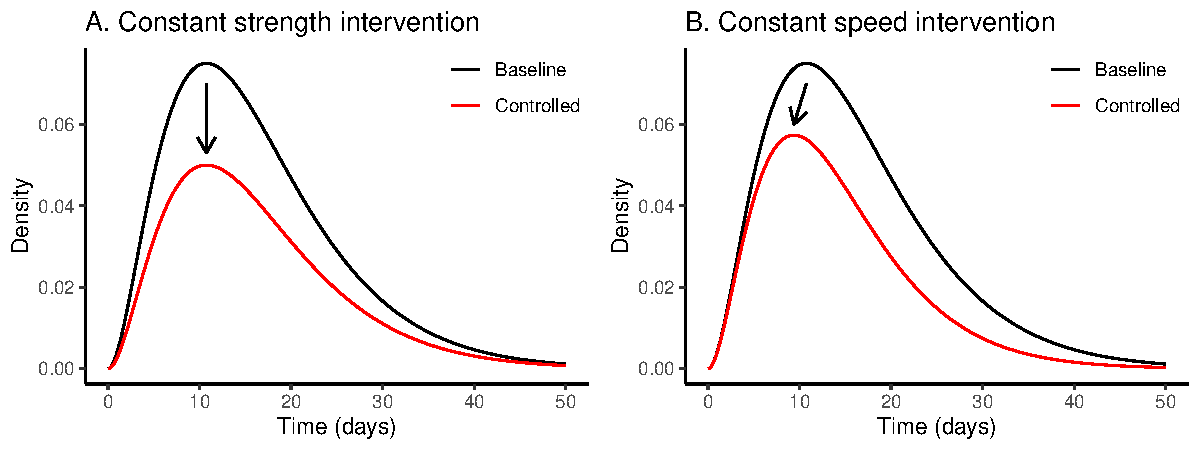
\includegraphics[width=\textwidth]{../figure/constant_intervention.pdf}
\caption{
\textbf{Effects of constant-strength and constant-speed intervention on infection kernels.}
Ebola-like gamma infection kernel $K(\tau)$ (mean: 16.2 days, CV: 0.58, and $\RR_0$: 1.5) is shown in black \citep{park2019practical}.
The infection kernel after applying each intervention strategy $\hat K(\tau)$ is shown in red.
(A) A constant-strength intervention with $\theta = 1.5$ is applied to an Ebola-like infection kernel.
A constant-strength intervention reduces the density by a constant proportion: $\hat K(\tau) = K(\tau)/\theta$; when the strength of intervention matches the strength of epidemic ($\theta = \mathcal R$), the resulting distribution is equivalent to the intrinsic generation-interval distribution ($\hat K(\tau) = g(\tau)$).
(B) A constant-speed intervention with $\phi \approx 0.0267/\mathrm{day}$ is applied to the same kernel.
A constant-speed intervention reduces the density exponentially: $\hat K(\tau) = K(\tau) \exp(-\phi \tau)$; when the speed of intervention matches the speed of epidemic ($\phi = r$), the resulting distribution is equivalent to the initial backward generation-interval distribution ($\hat K(\tau) = b(\tau)$). 
}
\figlab{constant}
\end{figure}

Assuming that the infection kernel $K$ doesn't change with time, we write:
\begin{equation}
	K(\tau) = \RR_0 g(\tau),
	\eqlab{strengthFactors}
\end{equation}
where $g(\tau)$ is the ``intrinsic'' generation-interval distribution.
The generation interval is defined as the time between when a person becomes infected and when that person infects another person \citep{svensson2007note};
therefore, the intrinsic generation-interval distribution $g(\tau)$ gives the relative infectiousness of an average individual as a function of time since infection \citep{champredon2015intrinsic}. 
Since $g$ is a distribution, it integrates to 1, and the basic reproductive number $\RR_0$ is thus the integral of $K$.

Imagine a control measure that proportionally reduces $K$, for example by protecting a fixed fraction of susceptibles through vaccination (\figref{constant}A). We then have:
\begin{equation}
	\hat K(\tau) = (\RR_0/\theta) g(\tau).
\end{equation}
Since $g$ is a distribution, the reduction needed to prevent invasion (or to eliminate disease)  is exactly $\theta=\RR_0$. We call $\theta$ the ``strength'' of the intervention; transmission is interrupted when the strength of the intervention $\theta$ is larger than the strength of spread $\RR_0$.

We generalize this idea by allowing an intervention strategy to reduce $K$ by different proportions over the course of an individual infection. We write the post-intervention kernel:
\begin{equation}
	\hat K(\tau) = K(\tau)/L(\tau), 
\end{equation}
where $L(\tau)$ is the average proportional reduction for an individual infected time $\tau$ ago.
The post-intervention reproductive number is thus:
\begin{equation}
	\Rhat = \int \hat K(\tau) d\tau
\end{equation}
This framework generalizes the work of \cite{fraser2004factors} who made parametric assumptions about the shape of $1/L(\tau)$.

We define the strength of the intervention $L$ to be $\theta = \RR_0/\Rhat$. It is then straightforward to show that $\theta$ is the harmonic mean of $L(\tau)$ weighted by generation-interval distribution:
\begin{equation}
	\theta = 1/\langle 1/L(\tau) \rangle_{g(\tau)}.
	\eqlab{strengthMean}
\end{equation}
In this more general case, we have again that the disease cannot spread when $\theta \geq \RR_0$.

\subsection{Speed-based decomposition}

The Euler-Lotka equation allows us to calculate the initial exponential growth rate $r$ of an epidemic given an infection kernel $K$:
\begin{equation}
	1 = \int K(\tau) \exp(-r\tau) d\tau
	\eqlab{euler}
\end{equation}
By analogy with the strength-based factorization \eqref{strengthFactors}, we can rewrite \eqref{euler} as a speed-based factorization:
\begin{equation}
K(\tau) = b(\tau)\exp(r\tau)
\end{equation}
Like $g$, $b$ is a distribution: in this case the initial backward generation interval, which gives the distribution of realized generation times (measured from the infectee's point of view) when the disease spreads exponentially \citep{champredon2015intrinsic, britton2019estimation}.

Now imagine an intervention that reduces transmission at a constant hazard rate $\phi$ across the disease generation (\figref{constant}B), for example by identifying and isolating infectious individuals.
We then have:
\begin{equation}
	\hat K(\tau) = K(\tau)\exp(-\phi\tau) = b(\tau)\exp((r-\phi)\tau)
\end{equation}
Since $b$ is a distribution (which integrates to 1), the reduction needed to prevent invasion (or to eliminate disease)  is exactly $\phi=r$. 
We call $\phi$ the ``speed'' of the intervention; transmission is interrupted when the speed of the intervention is faster than the speed of spread.

We generalize this idea by allowing the hazard rate $h(\tau)$ at which $K$ is reduced to vary through time, thus:
\begin{equation}
	\hat K(\tau) = K(\tau) \exp\left(-\int_0^\tau h(\sigma) d\sigma\right)
\end{equation}
The associated post-intervention epidemic speed $\hat r$ is given by:
\begin{equation}
	1 = \int \hat K(\tau) \exp(-\hat r\tau) d\tau.	
\end{equation}
We define the speed of a general intervention to be $\phi = r - \hat r$. 
We can then show that $\phi$ is a (sort of) mean satisfying:
\begin{equation}
	1 = \left\langle \frac{\exp(\phi \tau) }{\exp\left(\int_0^\tau h(\sigma) d\sigma\right)} \right\rangle_{b(\tau)}
	\eqlab{speedMean}
\end{equation}
Specifically, the speed $\phi$ is a mean of the hazard $h$ in the sense that an increase (or decrease) in $h$ produces the same sign of change in $\phi$, and if $h$ is constant across the generation then $\phi=h$.

\section{Example: Human immunodeficiency virus (HIV)}

\jd{I'd like to be even less detailed about HIV, and maybe do an explicit comparison with measles or Ebola. The idea I'd love to get across is that the two ways of thinking can both be helpful to intuition, and that which one fits better will depend on the disease and on the available data. I will work on making that part explicit.}

In this section, we use both strength- and speed-based decompositions to compare different intervention strategies for the human immunodeficiency virus (HIV). 
These examples are not meant to provide specific estimates of the effectiveness of intervention strategies; 
instead, we use these examples to demonstrate how strength- and speed-based decompositions can help us better evaluate control strategies under different scenarios.
In particular, we study how the amount of early HIV transmission affects our decision.

We model the infection kernel of the HIV as a sum of two gamma distributions:
\begin{equation}
K(\tau) = \mathcal R \left(\tsub{p}{early} \tsub{f}{early}(\tau) + (1-\tsub{p}{early}) \tsub{f}{late}(\tau) \right).
\end{equation}
The first component, $\tsub{f}{early}(\tau)$, models early HIV transmission during the acute infection stage.
We assume that $\tsub{f}{early}(\tau)$ has a mean of 3 months \citep{hollingsworth2008hiv} and a shape parameter of 3.
The second component, $\tsub{f}{late}$, models HIV transmission during the asymptomatic stage and the disease stage (after progression to Acquired Immune Deficiency Syndrome (AIDS)).
We assume that $\tsub{f}{late}(\tau)$ has a mean of 10 years \citep{brookmeyer1989censoring, nishiura2019estimating} and a shape parameter of 2 (this vaguely approximates the wide generation-interval distribution of the HIV \citep{fraser2004factors}).
Finally, $\tsub{p}{early}$ is the proportion of early HIV transmission.

\begin{figure}[!th]
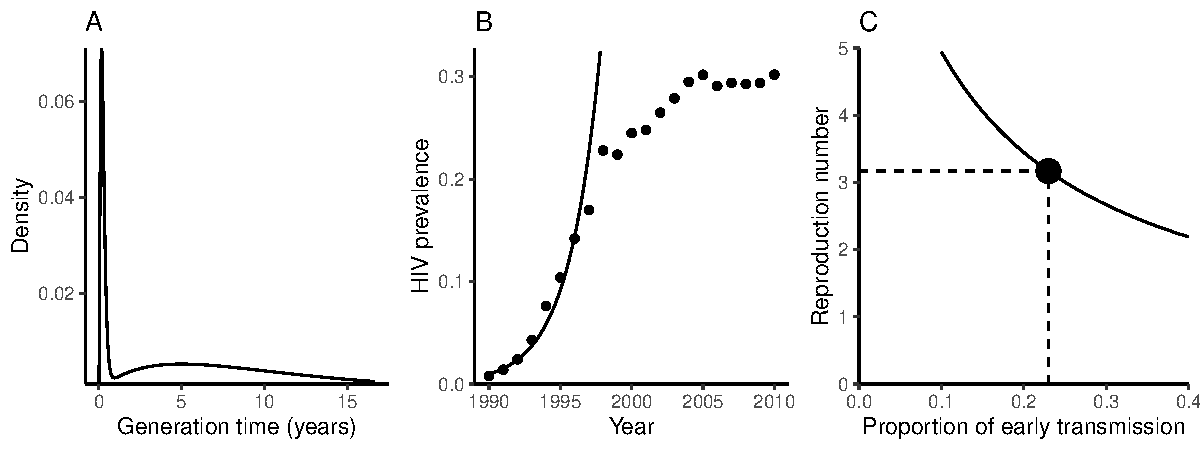
\includegraphics[width=\textwidth]{../figure/HIV.pdf}
\caption{
\textbf{The infection kernel of the HIV.}
(A) The infection kernel of the HIV is approximated using a sum of two gamma distributions. We assume that the baseline proportion of early transmission is 23\% \citep{hayes2006amplified}.
(B) Time series of HIV prevalence in pregnant women in South Africa, 1990 - 2010 \citep{barron2013eliminating}. The initial exponential growth rate of the HIV is estimated by fitting a straight line to log-prevalence (1990 - 1997) by minimizing the sum of squares.
(C) Increase in the estimate of the amount of early transmission reduces the estimate of the reproductive number.
The black circle indicates the baseline scenario.
}
\figlab{example}
\end{figure}

As our baseline scenario (\figref{example}A), we assume that early transmission is responsible for 23\% of the total transmission \citep{hayes2006amplified}.
Based on the growth rate estimate ($0.452\,\mathrm{year}^{-1}$; \figref{example}B) from HIV prevalence in pregnant women in South Africa \citep{barron2013eliminating}, our baseline reproductive number is $3.17$.
Increase in the estimate of the amount of early transmission shortens the mean generation time, which in turn decreases the reproductive number (\figref{example}C).
Therefore, we expect stronger (but not necessarily faster) intervention to be required in order to control the disease when there is less early transmission.

First, we consider a condom intervention that reduces HIV transmission by approximately 75\% at the population level.
Assuming that condoms act as a physical barrier, and that condom use will on average remain roughly constant through time, it is reasonable to model the proportional reduction in transmission due to condom use as constant across the course of infection: $\tsub{L}{condom} = 1/(1-0.75) = 4$  (\figref{condom}A).
The estimated strength of such an intervention is simply the average of $\tsub{L}{condom}$: $\theta=4$, whereas the estimated strength of the epidemic decreases as the proportion of early transmission increases (\figref{condom}B).
Thus, the predicted effectiveness of the condom intervention will depend strongly on our estimate of the importance of early transmission: if early transmission is low, we expect disease spread to be too strong to be controlled completely by our intervention.

\begin{figure}[!t]
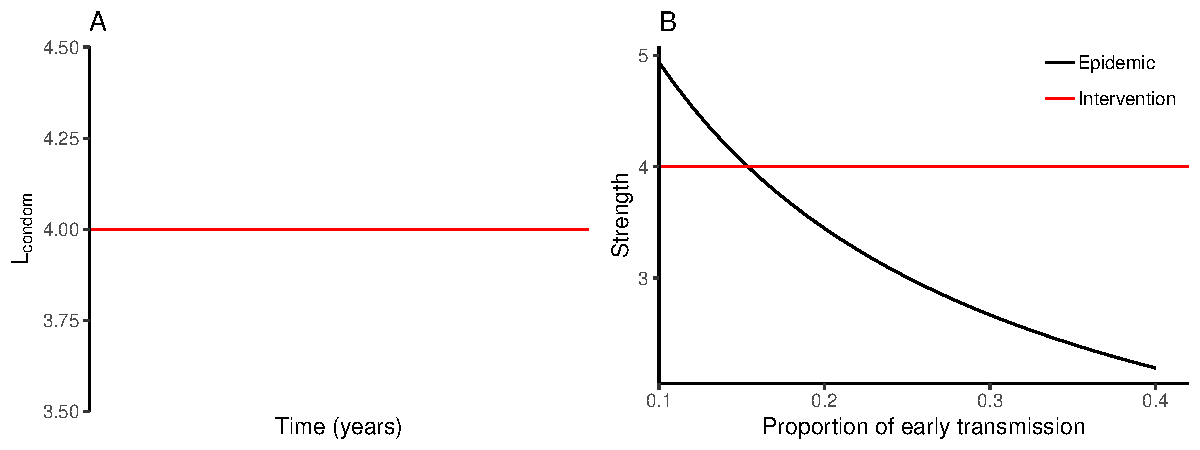
\includegraphics[width=\textwidth]{../figure/condom.pdf}
\caption{
\textbf{Understanding condom intervention using strength-based decomposition.}
(A) Condom use is thought to reduce probability of transmission by a similar factor throughout the course of infection; thus the proportional reduction $\tsub{L}{condom}$ due to condom use is constant across the course of infection.
(B) The estimated amount of early transmission affects estimated strength of the epidemic but not of a condom-based intervention.
The black and red circles indicate the baseline scenario.
}
\figlab{condom}
\end{figure}


\begin{figure}[!t]
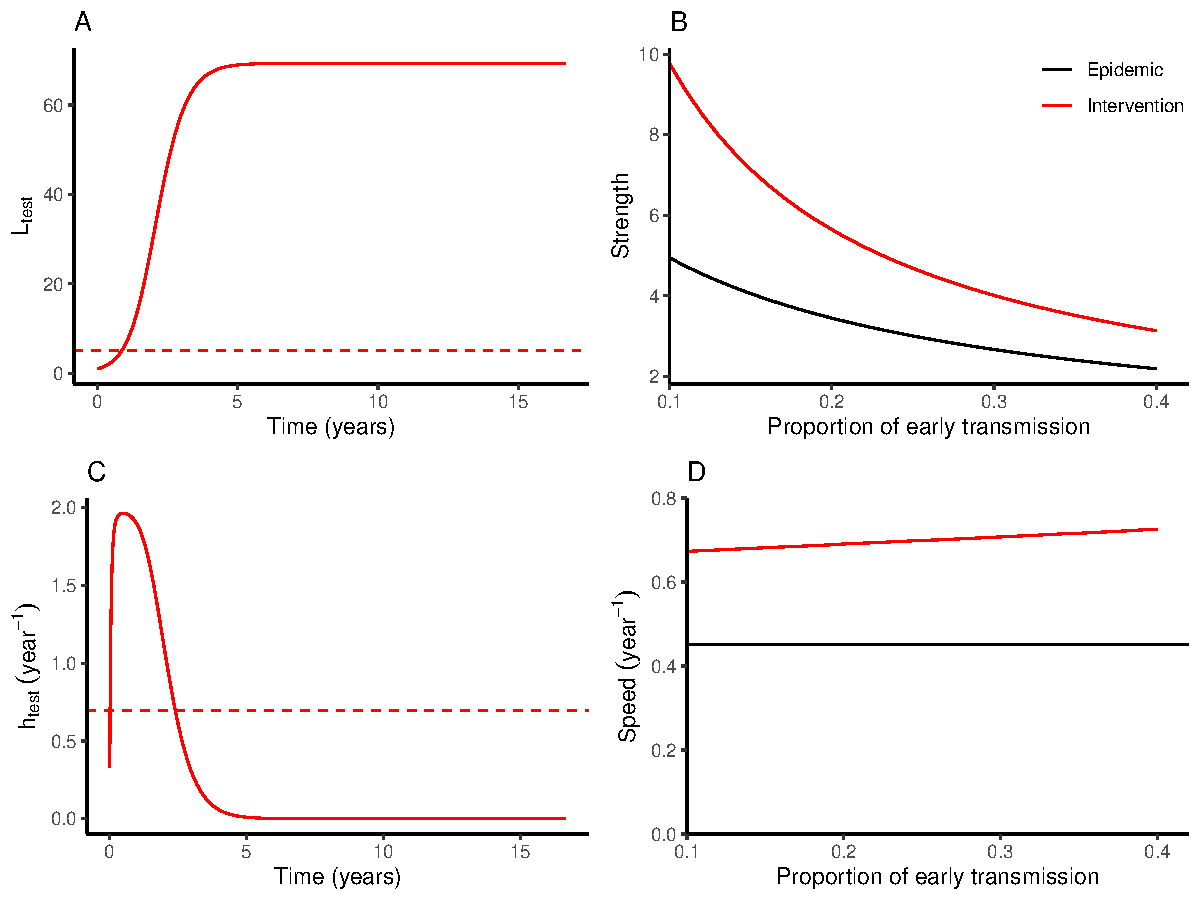
\includegraphics[width=\textwidth]{../figure/test_and_treat.pdf}
\caption{
\textbf{Understanding test-and-treat intervention using strength- and speed-based decomposition.}
\swp{We should just say exponentially. I see where you're coming from but the super-exponentiality seems negligible. Plotting on a log scale shows that it's approximately linear.}
(A) The effectiveness of test-and-treat intervention is assumed to increase super-exponentially at first, and then saturate. The dashed line shows the corresponding effective strength of the intervention (from \eqref{strengthMean}) assuming 23\% early transmission.
(B) Increase in the estimated amount of early transmission decreases the estimated strength of an epidemic as well as the estimated strength of test-and-treat intervention.
(C) The hazard rate correesponding to the strength curve in (A). 
The dashed line shows the corresponding effective speed of the intervention (from \eqref{speedMean}) assuming 23\% early transmission.
(D) The estimated amount of early transmission does not affect the observed speed of an epidemic but affects the estimated speed of intervention.
The black and red circles indicate the baseline scenario.
Test-and-treat intervention is modeled phenomenologically: $\tsub{L}{test}(\tau) = \exp\left(\int_0^\tau \tsub{h}{test}(\sigma) d\sigma \right)$ and $\tsub{h}{test}(\tau) = \tsub{h}{max} (1 - \exp(- K f(\tau)))$, where $f(\tau)$ is a gamma probability density function with a mean of $1$ year and a shape parameter of 2, $K = 4/\max(f(\tau))$, and $\tsub{h}{max} = 2\,\mathrm{year}^{-1}$.
}
\figlab{test}
\end{figure}

On the other hand, consider a ``test-and-treat'' strategy in which infected individuals are identified and put to clinical care, such as antiretroviral therapy (ART) \citep{garnett2009treating, nah2017test}.
We assume that the rate of identification and removal is initially constant.
Thus, the proportion continuing to transmit declines exponentially, and the effect of intervention $\tsub{L}{test}$ increases exponentially.
However, we assume removal eventually saturates, to account for the effects of people who avoid identification, persistent treatment failures, and the possibility of rare transmission even under effective treatment
(\figref{test}A; see caption for the functional form of $\tsub{L}{test}$).
Under this assumption, the strength of intervention decreases with the proportion of early transmission in a manner roughly similar to the epidemic strength.
In this scenario, we predict that the intervention remains effective over the range of considered parameters.

Using the speed-based decomposition allows us to understand the situation much more clearly.
The hazard rate $\tsub{h}{test}$ of this intervention starts at 0 (because infected individuals don't have a way to know that they have HIV when they're infected) but peaks very fast (because sexually active individuals are the most likely to seek testing); 
the assumed hazard rate goes down after a few months to reflect the satuaration assumptions discussed above. 
The speed of epidemic stays constant regardless of the proportion of the early transmission because epidemic speed corrresponds to the observed growth rate.
The speed of intervention stays roughly constant but slightly increases as proportion of early transmission increases because the subpopulation that the intervention fails to reach become relatively more important if late transmission is more important.
This framework provides an intuitive underpinning for the originally surprising result of \cite{eaton2014proportion}: the effectiveness of test-and-treat interventions should not depend much on the proportion of early transmission because early transmission has no effect on the estimated speed of the epidemic, and little on the estimated speed of the intervention.

\section{Discussion}

The effectiveness of an epidemic intervention is often measured by its ability to reduce the basic reproductive below 1.
In this study, we extend this idea by defining the strength of an intervention on the same scale as the strength of an epidemic (i.e., basic reproductive number $\mathcal R_0$) and the speed of an intervention on the same scale as the speed of an epidemic (i.e., exponential growth rate $r$).
We show that an intervention can successfully contain an epidemic if either its strength or speed is greater than their corresponding measures of the epidemic.

We compare two HIV intervention strategies (condom intervention and test-and-treat intervention) to demonstrate that both strength- and speed-based frameworks can be useful in evaluating the effectiveness of an epidemic intervention.
In particular, we recapitulate the result of \cite{eaton2014proportion} who used detailed mathematical modeling of HIV transmission to show that the amount of early transmission does not affect the effectiveness of the ART.
While they gave a strength-based argument for the result --  increasing the amount of early transmission decreases the basic reproductive number, which negatively correlates with the outcome of the ART intervention \citep{eaton2014proportion} -- there is a simple speed-based intuition behind this phenomenon: in principle, we can control the outbreak if we can identify infected individuals and put them on ART faster than the \emph{observed} rate at which new cases are generated, which does not depend on the amount of early transmission.
While both strength- and speed-based frameworks give the same conclusion about the outcome of an intervention, one can provide a clearer interpretation of the outcome than the other, depending on the situation.

The contrast between strength- and speed-based perspectives in characterizing an epidemic and its control can be widely found in studies of the West African Ebola Outbreak in 2014.
Early in the outbreak, many researchers tried to estimate the basic reproductive number and made policy suggestions based on their estimates \citep{althaus2014estimating, fisman2014early, gomes2014assessing, pandey2014strategies, shaman2014inference, towers2014temporal, who2014ebola}.
For example, \cite{pandey2014strategies} estimated $\mathcal R_0$ for the Liberian outbreak to be 1.63 and calculated that restricting post-burial transmission can reduce $\mathcal R_0$ below 1 but restricting hospital and community transmission cannot.
While these calculations are purely strength-based, these intervention strategies have both strength- and speed-like components: the effectiveness of safe burial practices depends on its ability to reduce the overall transmissibility (strength-like) as well as the amount of time it takes for a deceased individual to be buried (speed-like).

\cite{weitz2015modeling} later demonstrated that the strength of the Ebola outbreak cannot be reliably estimated early in an outbreak.
Instead, its speed can be directly measured from the incidence time series \citep{chowell2003sars, mills2004transmissibility, nishiura2009transmission, nishiura2010pros, ma2014estimating} and can provide a better framework for understanding the initial spread.
Many intervention strategies that played major role in controlling the Ebola outbreak were, in fact, speed-like: identifying and isolating infected individuals, contact-tracing, etc. \citep{pandey2014strategies}.
Like the test-and-treat intervention for HIV, the effectiveness of these strategies would not have depended on the uncertainty in the underlying disease generation time (which would have been propagated from the uncertainty in the amount of post-burial transmission).



\bibliography{speedstrength}

\end{document}
